\chapter{Title of the appendix 1}
\label{chap:appendix1}
%Reducing the spacing from the title


Here you write the context of the appendix, structuring such content in
sections, sub-sections and sub-sub-sections, if needed.

An example of appendix is the flat presentation of all the graphical user interface screens.
Each screen can be presented (identification symbol and description) and screens transition graph can be given.


\section{My Section}
\label{sec:appendix1_mySection}
Description of the section.



\subsection{My subSection}

\subsubsection{My subSubSection}


\section{Graphical User Interface screens}

%=======================Admin Control Panel============================
\subsection{Administrator Control Panel}

\begin{figure}
  \centering
    
\includegraphics{images/mockups/feature1-login/AdminLogon.eps}
  \caption{Administrator login}
  \label{fig:AdminLogin}
\end{figure}


\begin{figure}
  \centering
    
\includegraphics{images/mockups/feature1-login/AdminConfirm.eps}
  \caption{Administrator confirm dialog}
  \label{fig:AdminConfirm}
\end{figure}


\begin{figure}
  \centering
    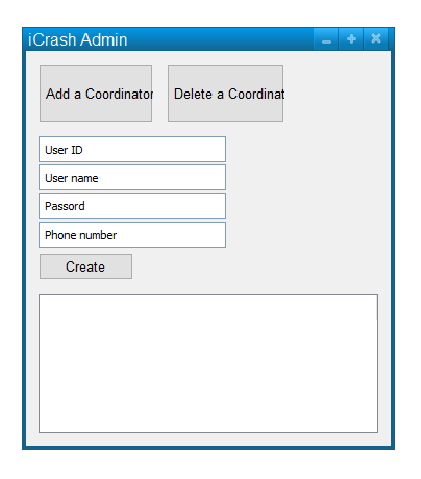
\includegraphics{images/mockups/feature1-login/AdminAddCoordinator.eps}
  \caption{Administrator add Coordinator window}
  \label{fig:AdminAddCoordinator}
\end{figure}


%=======================Coordinator Control Panel============================
\subsection{Coordinator Control Panel}

\begin{figure}
  \centering
    
\includegraphics{images/mockups/feature1-login/CoordinatorLogon.eps}
  \caption{Coordinator login}
  \label{fig:CoordinatorLogin}
\end{figure}


\begin{figure}
  \centering
    
\includegraphics{images/mockups/feature1-login/CoordinatorConfirm.eps}
  \caption{Coordinator confirm dialog}
  \label{fig:CoordinatorConfirm}
\end{figure}
%==================SMS conversation between Victim and System=================
\subsection{SMS conversation between Victim and iCrash System}

\begin{figure}
  \centering
    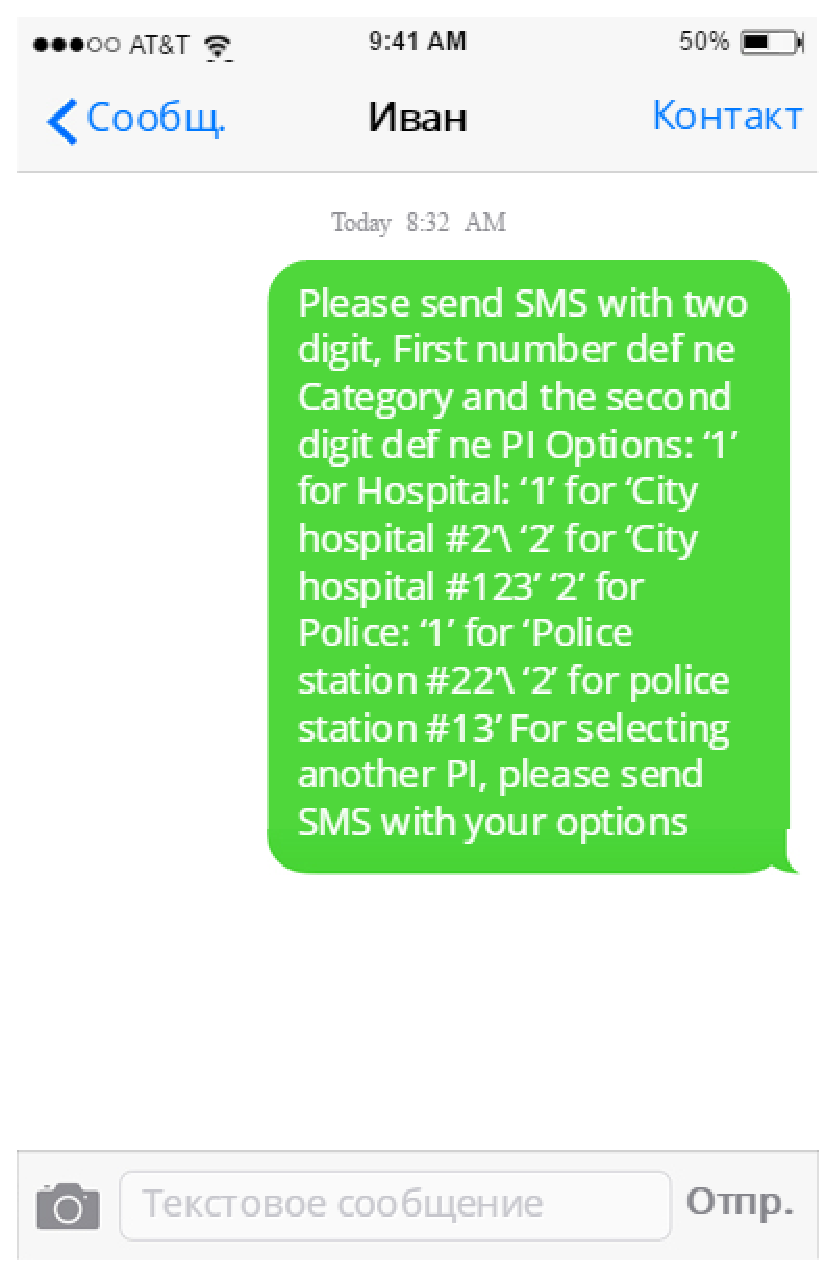
\includegraphics[width=6cm]{images/mockups/feature3-PI/1.eps}
  \caption{Select category}
  \label{fig:Selectcategory}
\end{figure}


\begin{figure}
  \centering
    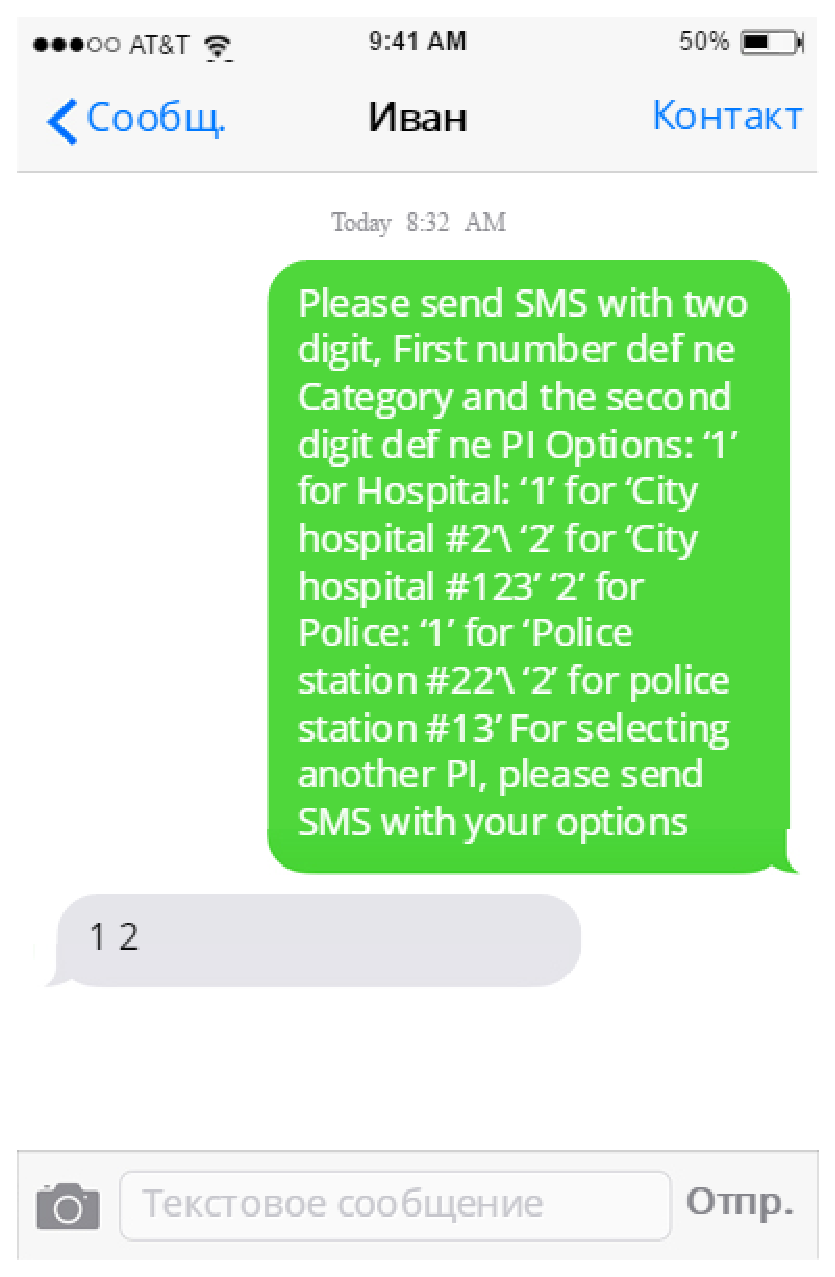
\includegraphics[width=6cm]{images/mockups/feature3-PI/2.eps}
  \caption{Victim choice}
  \label{fig:Victimchoice}
\end{figure}  


\begin{figure}
  \centering
    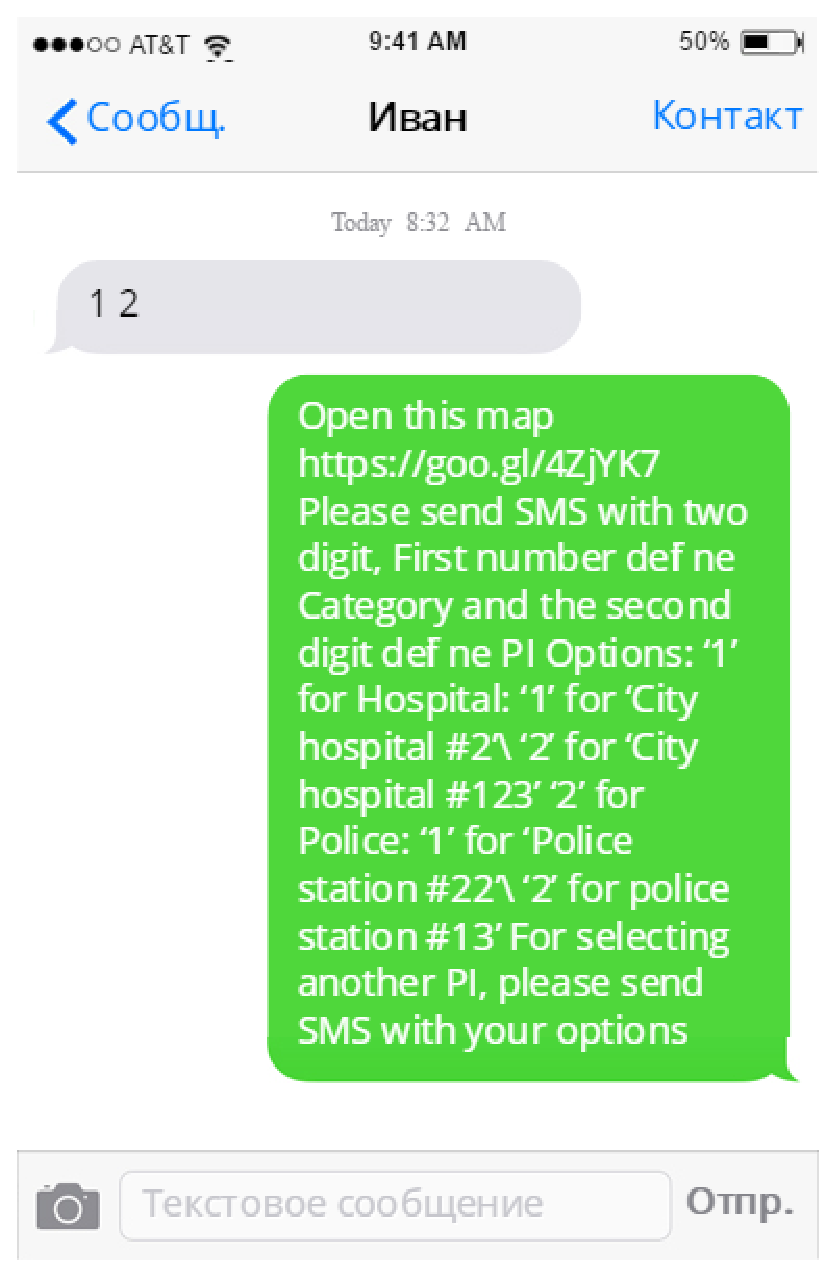
\includegraphics[width=6cm]{images/mockups/feature3-PI/3.eps}
  \caption{Answer on selection}
  \label{fig:Answeronselection}
\end{figure}


